% This is samplepaper.tex, a sample chapter demonstrating the
% LLNCS macro package for Springer Computer Science proceedings;
% Version 2.20 of 2017/10/04
%
\documentclass{llncs}
%
\usepackage{graphicx}
\usepackage{float}
% Used for displaying a sample figure. If possible, figure files should
% be included in EPS format.
%
% If you use the hyperref package, please uncomment the following line
% to display URLs in blue roman font according to Springer's eBook style:
% \renewcommand\UrlFont{\color{blue}\rmfamily}

\begin{document}
%
\title{ImageCLEF 2019: Deep Learning for Tuberculosis CT Image Analysis}
%
%\titlerunning{Semantic descriptors for Tuberculosis patients}
% If the paper title is too long for the running head, you can set
% an abbreviated paper title here
%
\author{Abdelkader Hamadi\orcidID{0000-0001-9990-332X} \and Noreddine Belhadj Cheikh \and Yamina Zouatine \and Si Mohamed Bekkai Menad \and Mohamed Redha Djebbara}




%
%\authorrunning{A. Hamadi et al.}
% First names are abbreviated in the running head.
% If there are more than two authors, 'et al.' is used.
%
\institute{University of Abdelhamid Ibn Badis Mostaganem\\Faculty of Exact Sciences and Computer Science\\Mathematics and Computer Science Department\\ Mostaganem, Algeria\\$\;$\\
\email{abdelkader.hamadi@univ-mosta.dz}\\
\email{noreddine.belhadjcheikh@univ-mosta.dz}\\
\email{zouatineyamina@gmail.com}\\
\email{bekkai.menad@univ-mosta.dz}\\
\email{redha.djebbara@univ-mosta.dz}
}




%
\maketitle              % typeset the header of the contribution
%
\begin{abstract}
In this article, we present our methodologies used in our participation to the two subtasks of the ImageCLEF 2019 Tuberculosis Task (SVR and CTR). Our contributions are essentially based on deep learning and other machine learning techniques. In addition to the use of deep learners, semantic descriptors are tested to represent patients CT scans. These features are extracted after a first learning step. Our submissions on the test corpus reached AUC value of about 65\% in the SVR task and 63\% in CTR. These results offered us the seventh and the eighth places in SVR and CTR, respectively. We believe that our contributions could be further improved and might give better results if they applied properly and in an optimized way.

\keywords{ImageCLEF \and Tuberculosis Task \and Deep Learning \and CT Image  \and Tuberculosis CT Image Classification \and Tuberculosis Severity Scoring \and CT Report.}
\end{abstract}
%
%
%
\section{Introduction}
Tuberculosis (TB) is a deadly disease. Its early diagnosis can give the necessary treatment and prevent the death of patients. The technological advancement especially in the field of artificial intelligence and precisely supervised learning opens the door for researchers to study the possibility of an automatic diagnosis. This would speed up the process and lower its cost. Several researchers have invested their efforts in recent years, especially within the medical image analysis community. In fact, a task dedicated to this disease had been adopted as part of the ImageCLEF evaluation campaign in its editions of the three last years~\cite{ImageCLEFTB2017,ImageCLEFTB2018,ImageCLEFTBoverview2019}. In this task, the objective is to automatically analyze the 3D CT images of TB patients to detect semantic information: the type of Tuberculosis, the degree of severity of the disease, information related to the state of the lungs, etc. In ImageCLEF 2019 two sub-tasks of the main task ``ImageCLEFmed Tuberculosis" are considered: Severity Scoring (SVR) and CT Report (CTR). In the first task, the goal is to deduce automatically from a CT image whether a TB case is severe or not. In the second one, the problematic consists to deduce automatically from the same type of image information about patient lungs state: which of the two lungs is affected, the presence of caverns, etc.\\


We can summarize the objectives of the Tuberculosis task through the following points:

\begin {itemize}
\item Helping medical doctors in the diagnosis and determining the state of the patient through image processing techniques;
\item Predicting quickly the TB severity degree to make quick decisions and give effective treatments;
\item Assist doctors and medical officers to have accurate details about the patient's lung condition by providing a report summarizing information describing the state of the lungs.
\end {itemize}

We present in the following our work that had been made in the context of our participation in the two sub-tasks of ImageCLEF 2019 Tuberculosis task: Tuberculosis Severity Scoring (SVR) and Tuberculosis CT Report (CTR)~\cite{ImageCLEFTBoverview2019}.\\

The remainder of this article is organized as follows. Section 2 describes the two tasks to which we had participated. In section 3, we present our contribution by detailing the system deployed to complete our submissions. Section 4 details our experimental protocols used to generate our predictions. We present and analyze in the same section the results obtained. We conclude in the last section by presenting some perspectives and future works.

\section{Participation to ImageCLEF 2019}

ImageCLEF 2019~\cite{ImageCLEF19} is an evaluation campaign that is being organized as part of the CLEF initiative labs. This campaign offers several research tasks that welcome participation from teams around the world. For the 2019 edition, ImageCLEF organises four main tasks: ImageCLEFcoral, ImageCLEFlifelog, ImageCLEFmedical and ImageCLEFsecurity. In this work, we focus on the Tuberculosis task that takes part in the ImageCLEFmedical challenge. ImageCLEFmed Tuberculosis task includes two sub-tasks: Severity Scoring (SVR) and CT Report (CTR) that we describe in the following.

\subsection{SVR and CTR Tasks description}
In this paper, we focus on our participation in the SVR and the CTR sub-tasks. The main objective of these two challenges is the automatic analysis of Tuberculosis CT scans. In both tasks, the same data collections are used, one corpus for training and another set for test. The data is provided as 3D CT scans. All the CT images are stored in NIFTI file format with ``nii.gz" extension file (gzipped .nii files). For each of the three dimensions of the CT image, we find a number of slices varying according to the dimension considered (512 images for the $Y$ and $X$ dimensions, from 40 to 250 images for the $Z$ dimension). Each slice has a size of about 512$\times$128 pixels for the $X$ and $Y$ dimensions and 512$\times$512 pixels for the $Z$ dimension.\\

A training collection is provided at the beginning of the task with its ground-truth (labels of samples). Participants prepare and train their systems on this dataset. A test collection is provided at a later date. Participants interrogate their system and return their predictions to the organizers' committee. An evaluation is performed by the latter to compare the performance of the submitted systems.

\subsubsection{SVR task}
aims to predict the degree of severity of TB cases. Given a CT scan of TB patient, the main goal is to predict the severity of his illness based on his 3D CT scan. The degree of severity is modeled according to 5 discrete values: from 1 (``critical/very bad") to 5 (``very good"). The score value is simplified so that values 1, 2 and 3 correspond to ``high severity" class, and values 4 and 5 correspond to ``low severity".

The classification problem is evaluated using two measures: 1) Area Under ROC-curve (AUC) and 2) Accuracy. 

\subsubsection{CT Report task} has as objective to automatically generate a report based on the patient's CT scan. This report should include the following six pieces of information in the binary form (0 or 1):
\begin{enumerate}
 \item is the left lung affected ?
 \item is the right lung affected ? 
\item the presence of calcifications;
 \item the presence of caverns;
  \item the presence of pleurisy;
 \item the lung capacity decrease.
\end{enumerate}

This task is considered as a multi-binary classification problem (6 binary findings). The ranking of this task is done first by average AUC and then by min AUC (both over the 6 CT findings).

\section{Our contributions}
\label{contribution}
We proposed to use the system presented in Figure~\ref{fig:system}. The latter goes through two essential steps: input data pre-processing and learning a classification model. A third optional step is added in order to improve the performance of the first learning step. The latter includes a second learning stage by using a recurrent neural network (LSTM) or by generating semantic features and exploiting them through a learner or a deep learner. We will detail our proposed system in the following.

\begin{figure}
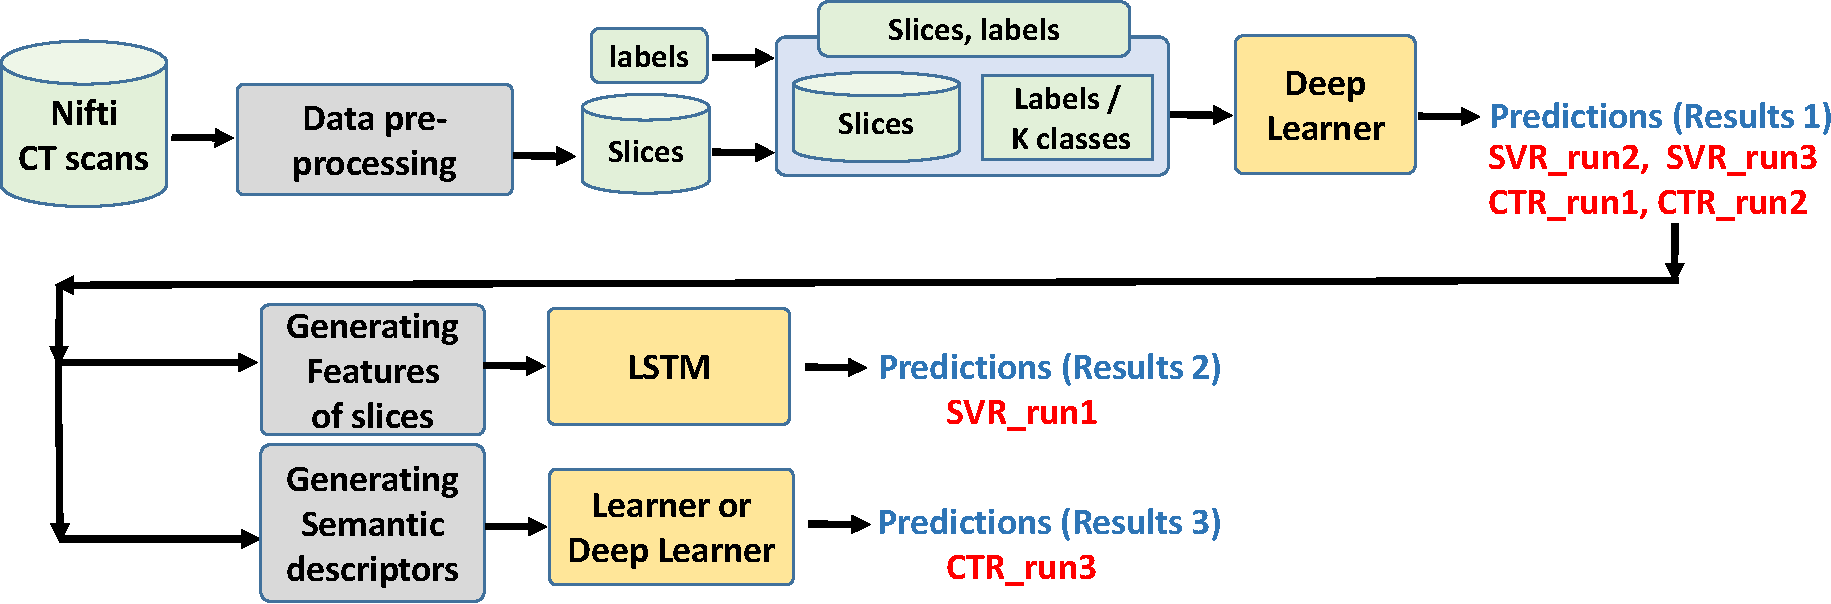
\includegraphics[width=\textwidth,height=6cm]{system.pdf}
\caption{The architecture of the overall proposed system} 
\label{fig:system}
\end{figure}


\subsection{Input data pre-processing}
\label{preprocess}
We remind that in both tasks, 3D CT scans are provided in compressed Nifti format. Firstly, we decompressed the files and extracted the slices. At the end, we got three sets of slices corresponding to the three dimensions of the 3D image. For each dimension and for each Nifti image we obtained a number of slices ranging according to the dimension considered (512 images for the $Y$ and $X$ dimensions, from 40 to 250 images for the $Z$ dimension).\\

The visual content of the images extracted from the different dimensions is not similar. Indeed, the images of each dimension are taken from a different angle of view. We noticed from our experiments that the slices of the -Z- dimension give better results compared to the two others (X and Y). This remark concerns our proposed approaches. This is why we used in our work the Z-dimension. However, all steps can be applied to slices of any of the three dimensions.\\

After choosing the dimension to consider, we propose to filter the slices of each patient. Indeed, we can notice that many slices do not necessarily contain relevant information that could help to classify the samples. This is why we added a step to filter and select a number of slices per patient. For this, we propose two filtering approaches:\\

\textbf{Automatic supervised filtering:} In this approach, we select a set of patients from each of the considered classes (the five degrees of severity for the SVR task). Then, a professional radiologist selects for each patient, the slices likely to contain relevant information indicating the presence of Tuberculosis. The resulting set of slices constitutes a filtering group. Given a new patient, we compare each of its slices to the filtering group by calculating a distance measure:  a weighted sum of distances between the slice and those of the filtering group. This comparison was made through a direct pixel-wise comparison. We selected at the end $N$ slices that are judged to be the most similar to the filtering group. So, at the end, each patient is represented by the $N$ filtered slices instead of all its extracted images. We think that this would reduce the noise introduced by the consideration of all slices. We tested in our contributions the value N=10.

\begin{figure}
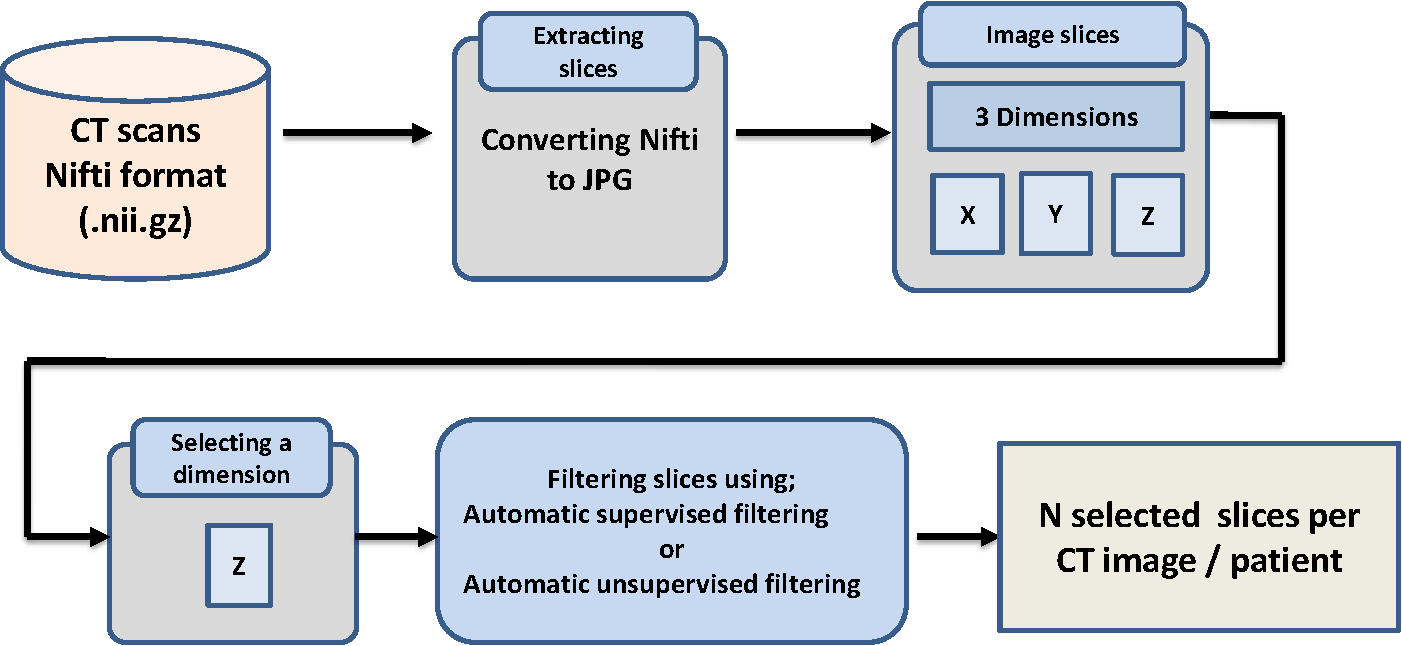
\includegraphics[width=\textwidth,height=4.5cm]{preprocess.pdf}
\caption{Pre-processing of input data.} 
\label{fig:preprocess}
\end{figure}

\textbf{Automatic unsupervised filtering:}
We noticed that there is usually a maximum of 50/60 slices visually informative. Since the slices are ordered, the most informative slices are usually at the center of the list. We propose then to keep only the $N$ middle ones. This is not optimal but we opted for this choice for a fully automatic and unsupervised approach. This choice can be improved by performing a manual filtering with the intervention of a human expert, preferably with medical skills on TB disease.\\

Figure~\ref{fig:preprocess} summarizes the pre-processing steps.

 
\subsection{Deep learning model for CT image classification (first learning step)}
As a deep learner, we chose to use Resnet-50 architecture because of its good results in the context of the same problematic in last Tuberculosis task editions~\cite{sgeast17}. On the other hand, we developed our model that we called ``LungNet". We present more details about this deep  learner in the following section. The outputs of the deep learners deployed are considered as initial results. We exploited then these outputs to generate : 1) semantic features of patient that are used to reclassify the samples, and 2) features of slices organized in a sequence format that are pushed to LSTM input as it is described in section~\ref{lstm}.\\

\textbf{LungNet Deep Learner:}
We proposed and developed our deep learner architecture for CT Image Analysis that we called ``LungNet''. The input to the latter is an RGB image of size 119x119, followed by five convolutional layers and two fully connected layers. Initially input data were in nifty format. Slices of the CT scans are 1-channel gray-level images. However,  we extracted the slices using med2image tool~\cite{med2image}. This software converts the slices to jpeg format. To avoid introducing noise by using this extraction method, we can do better by reading directly image pixels values using Niftilib library for python that was suggested by the task organizers. The idea behind using med2image to extract slices is that we planned to filter the slices by a medical expert intervention. This process needs to sees the content of slices. 


\begin{figure}
%\vspace{-2cm}
\center
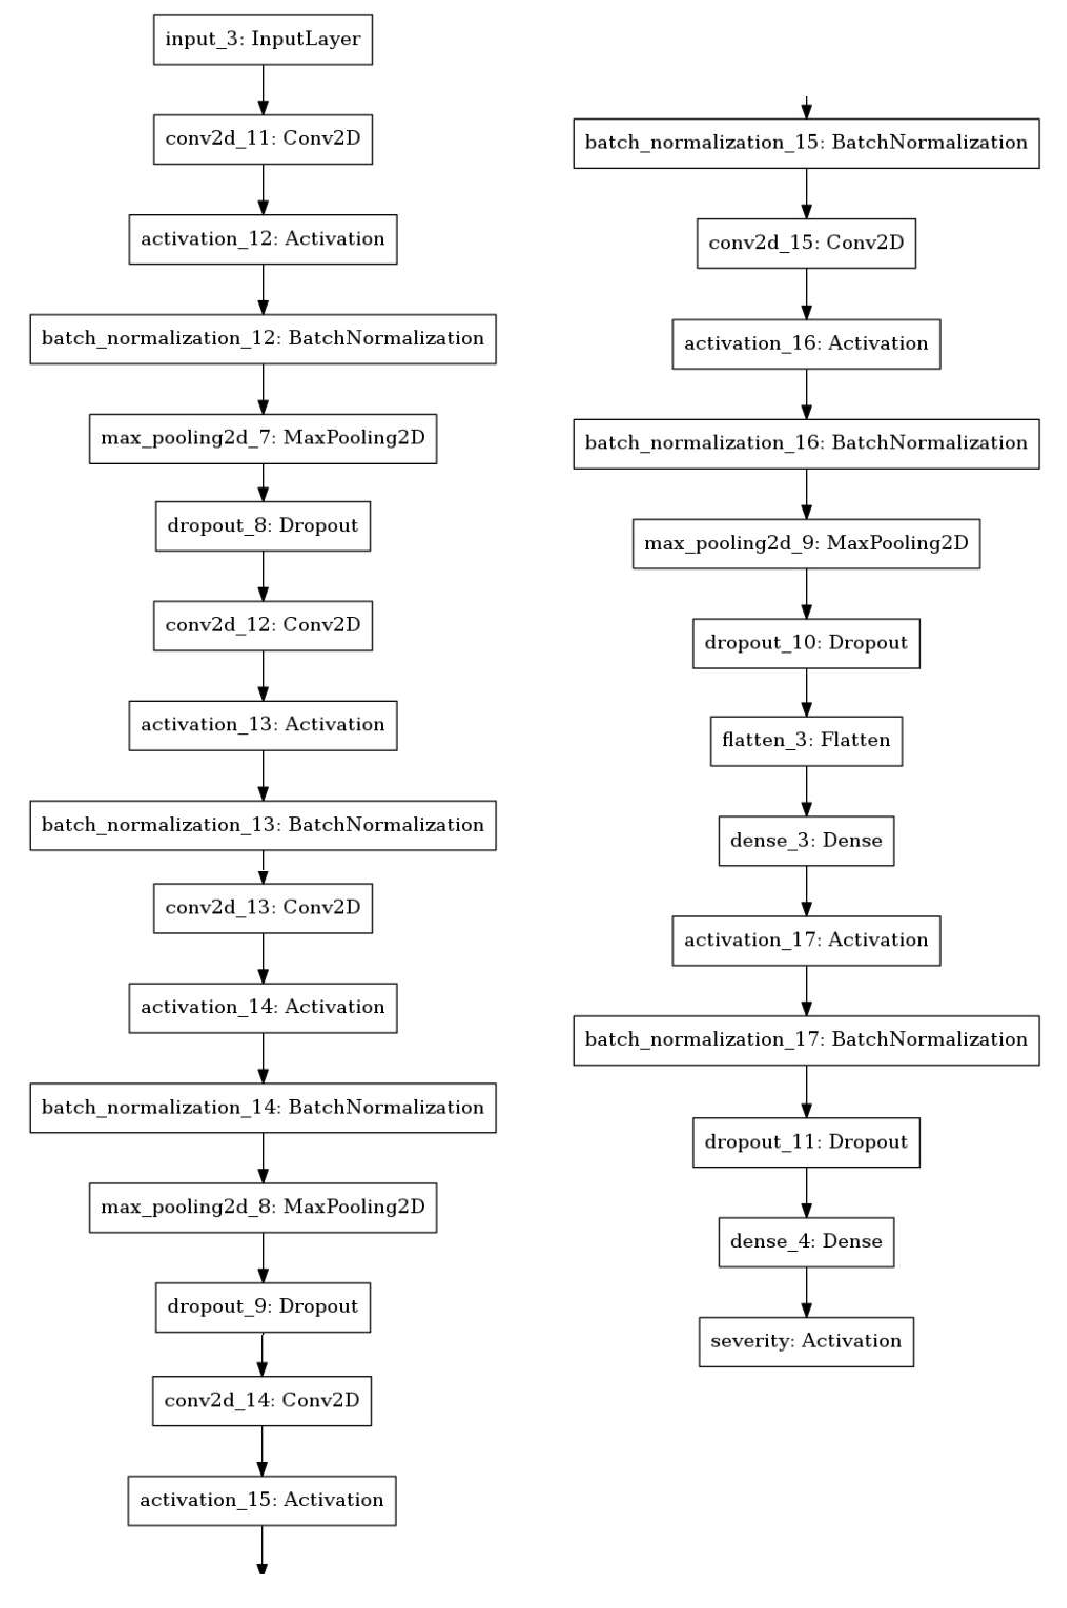
\includegraphics[width=10cm,height=10cm]{lungnet3.pdf}
\caption{The architecture of the LungNet Deep Learner} 
\label{fig:lungnet}
\end{figure}


After each convolutional layer ``relu" activation is applied followed by a local normalization and MaxPooling. The first, the second and the third convolution blocks have dropout layers to reduce overfitting. The sigmoid activation function is applied to the output layer in order to predict values in the range of 0 to 1.\\

Figure~\ref{fig:lungnet} illustrates the architecture of the Lungnet model.





\subsection{Semantic Features extraction}
\label{semDesc}
We implemented the method of semantic descriptors extraction described in~\cite{HamadiY18} with slight differences. After slices extraction and filtering, we generated a single descriptor per patient to exploit it through a transfer learning process. The results of SGEast~\cite{sgeast17} and even other teams in the same task of ImageCLEF 2017 proved the efficiency of this approach~\cite{sgeast17,HamadiY18}.

\begin{figure}[!ht]
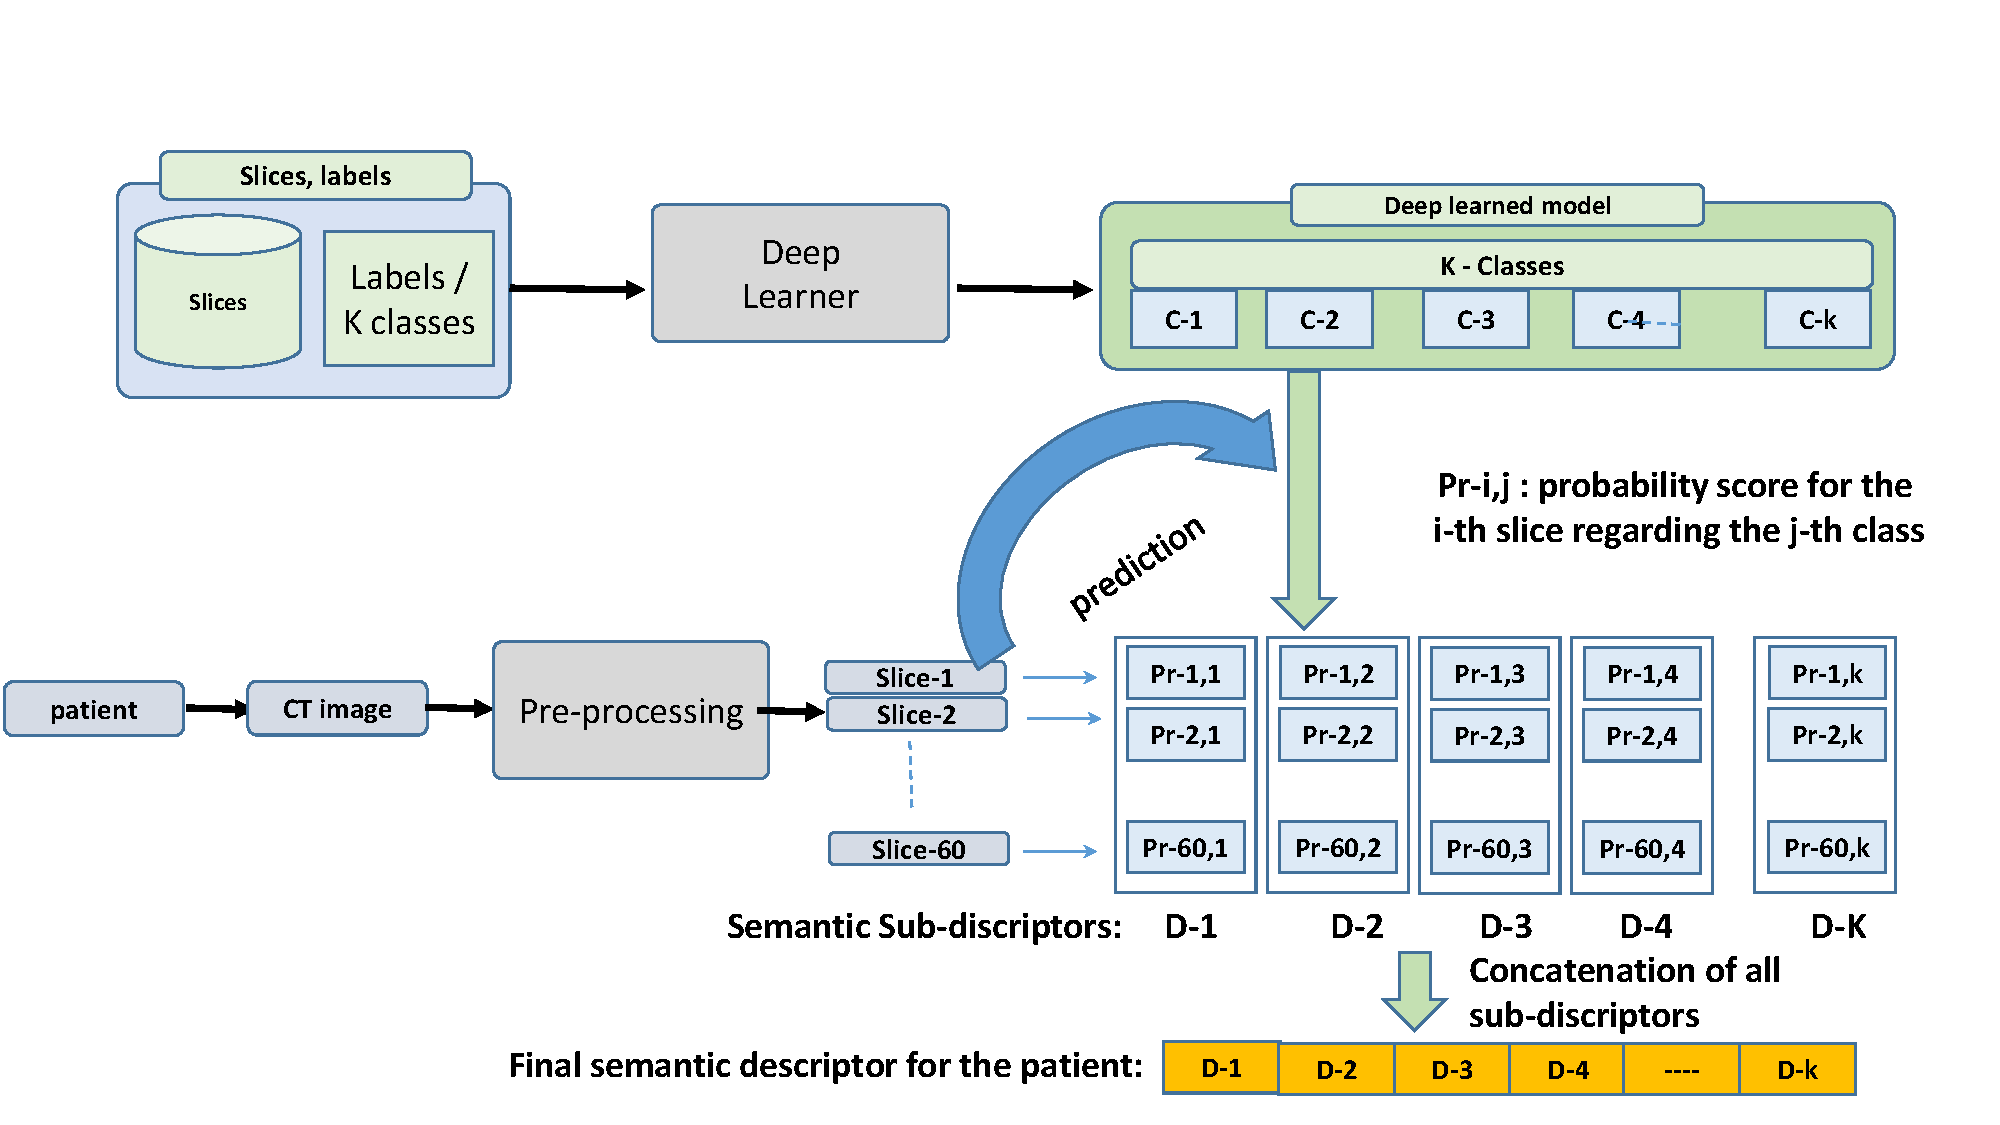
\includegraphics[width=\textwidth,height=8cm]{semanticFeatures.pdf}
\caption{Semantic features extraction process~\cite{HamadiY18}.} 
\label{fig:semanticFeatures}
\end{figure}

So, we chose to exploit the probabilities predicted by a deep learner trained on a set of slices. If $K$ is the number of classes considered, these predictions typically correspond to the $K$ predicted probability values ​​for the $K$ classes (For SVR Task, $K=5$: the five severity degrees). We obtain then for each slice $K$ values ​​corresponding to the probabilities of the $K$ considered classes.\\


Furthermore, $K$ sub-descriptors are generated: $D_1$, $D_2$, $D_3$, $D_4$, ... $D_k$. Each sub-descriptor $D_i$ contains the predicted probabilities for the class $i$ for all the slices of the patient. A final semantic descriptor is constructed by concatenating the $K$ sub-descriptors. Figure~\ref{fig:semanticFeatures} details the whole process of the semantic features extraction for one patient.




\subsection{Learning a classification model based on semantic features (second learning step)}
We propose to exploit the semantic descriptors of patients described previously. Any approach of supervised classification can be applied as shown in figure~\ref{fig:classification}. We tested in our experiments SVM as supervised classifier. However, Random Forests and bagging of Random Forests have shown good results in the context of the same problematic~\cite{HamadiY18}.\\

\begin{figure}[!ht]
\center
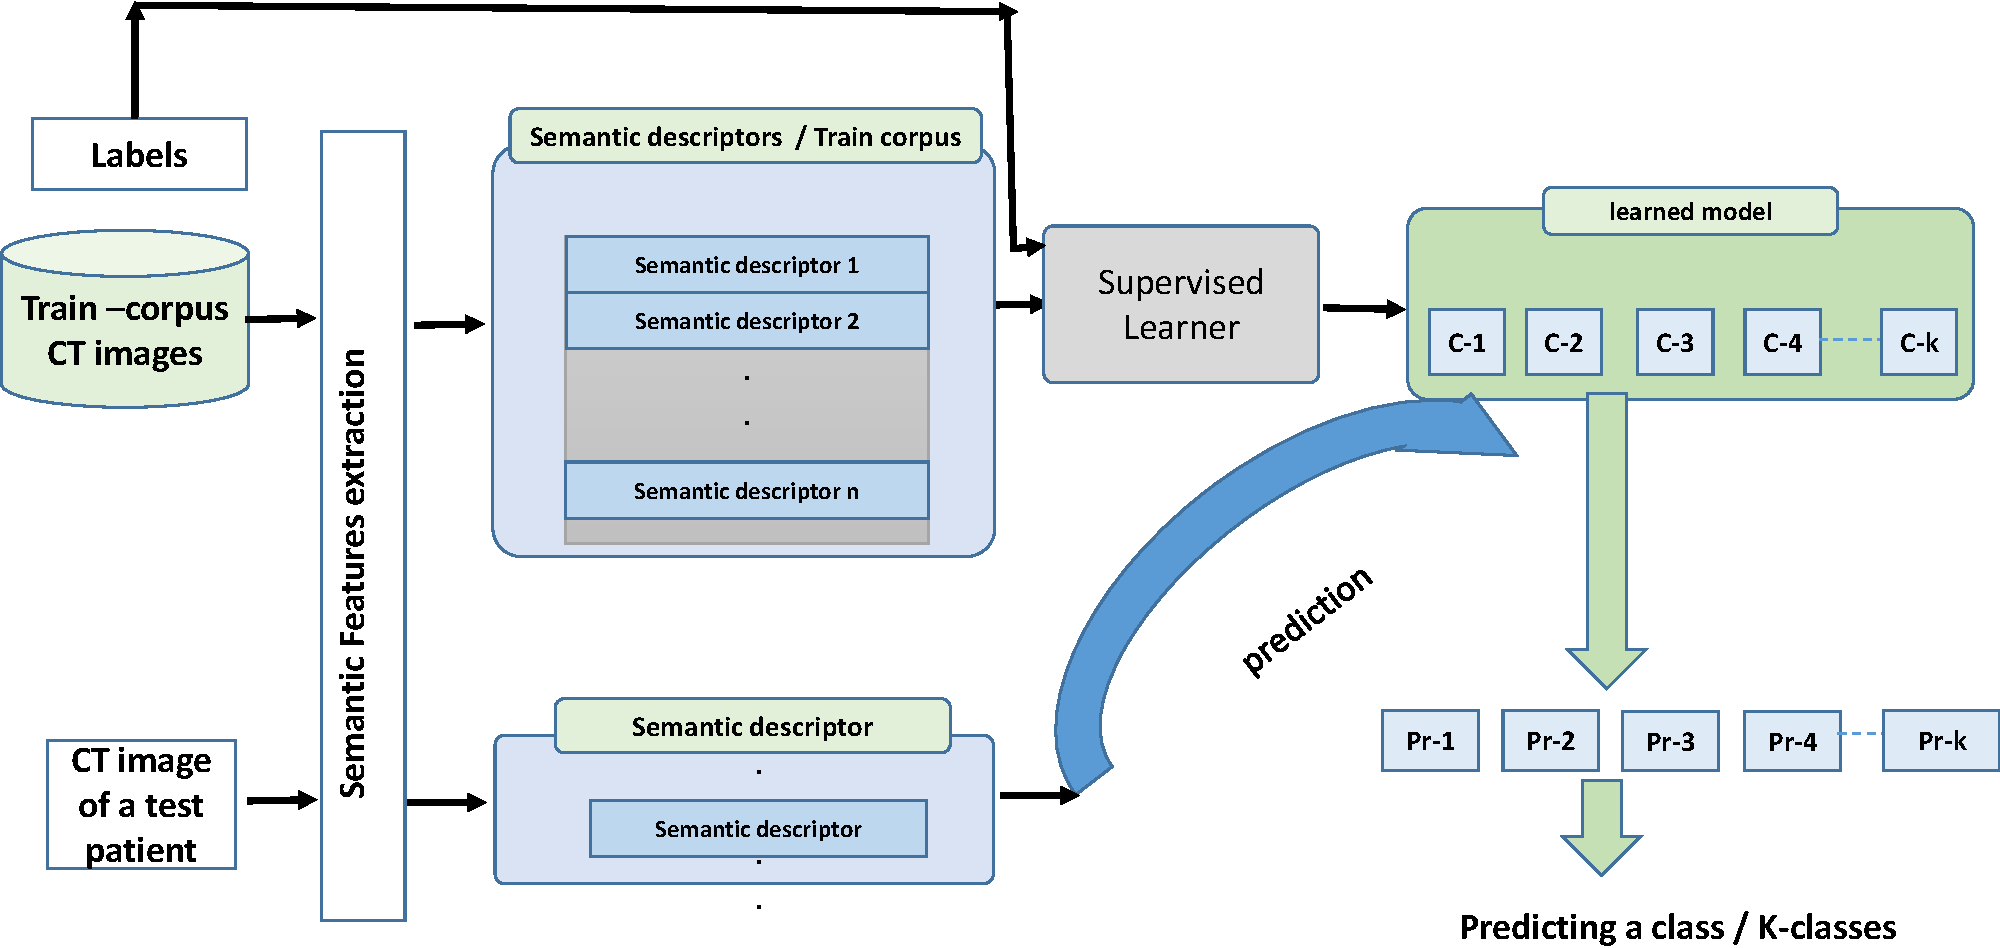
\includegraphics[width=\textwidth,height=8cm]{classification.pdf}
\caption{Learning a classification model based on the semantic descriptors~\cite{HamadiY18}.} 
\label{fig:classification}
\end{figure}

We recommend some ideas for this step:
\begin{itemize}
\item To use a deep learner having as input the semantic descriptors of patients and their labels. As an alternative, it would be interesting to use a bagging method that collaborates several learners and sub-samples the train collection. This would lead to better results as presented in~\cite{HamadiY18};
\item To apply samples selection and data augmentation.
\end{itemize}


\begin{figure}[!ht]
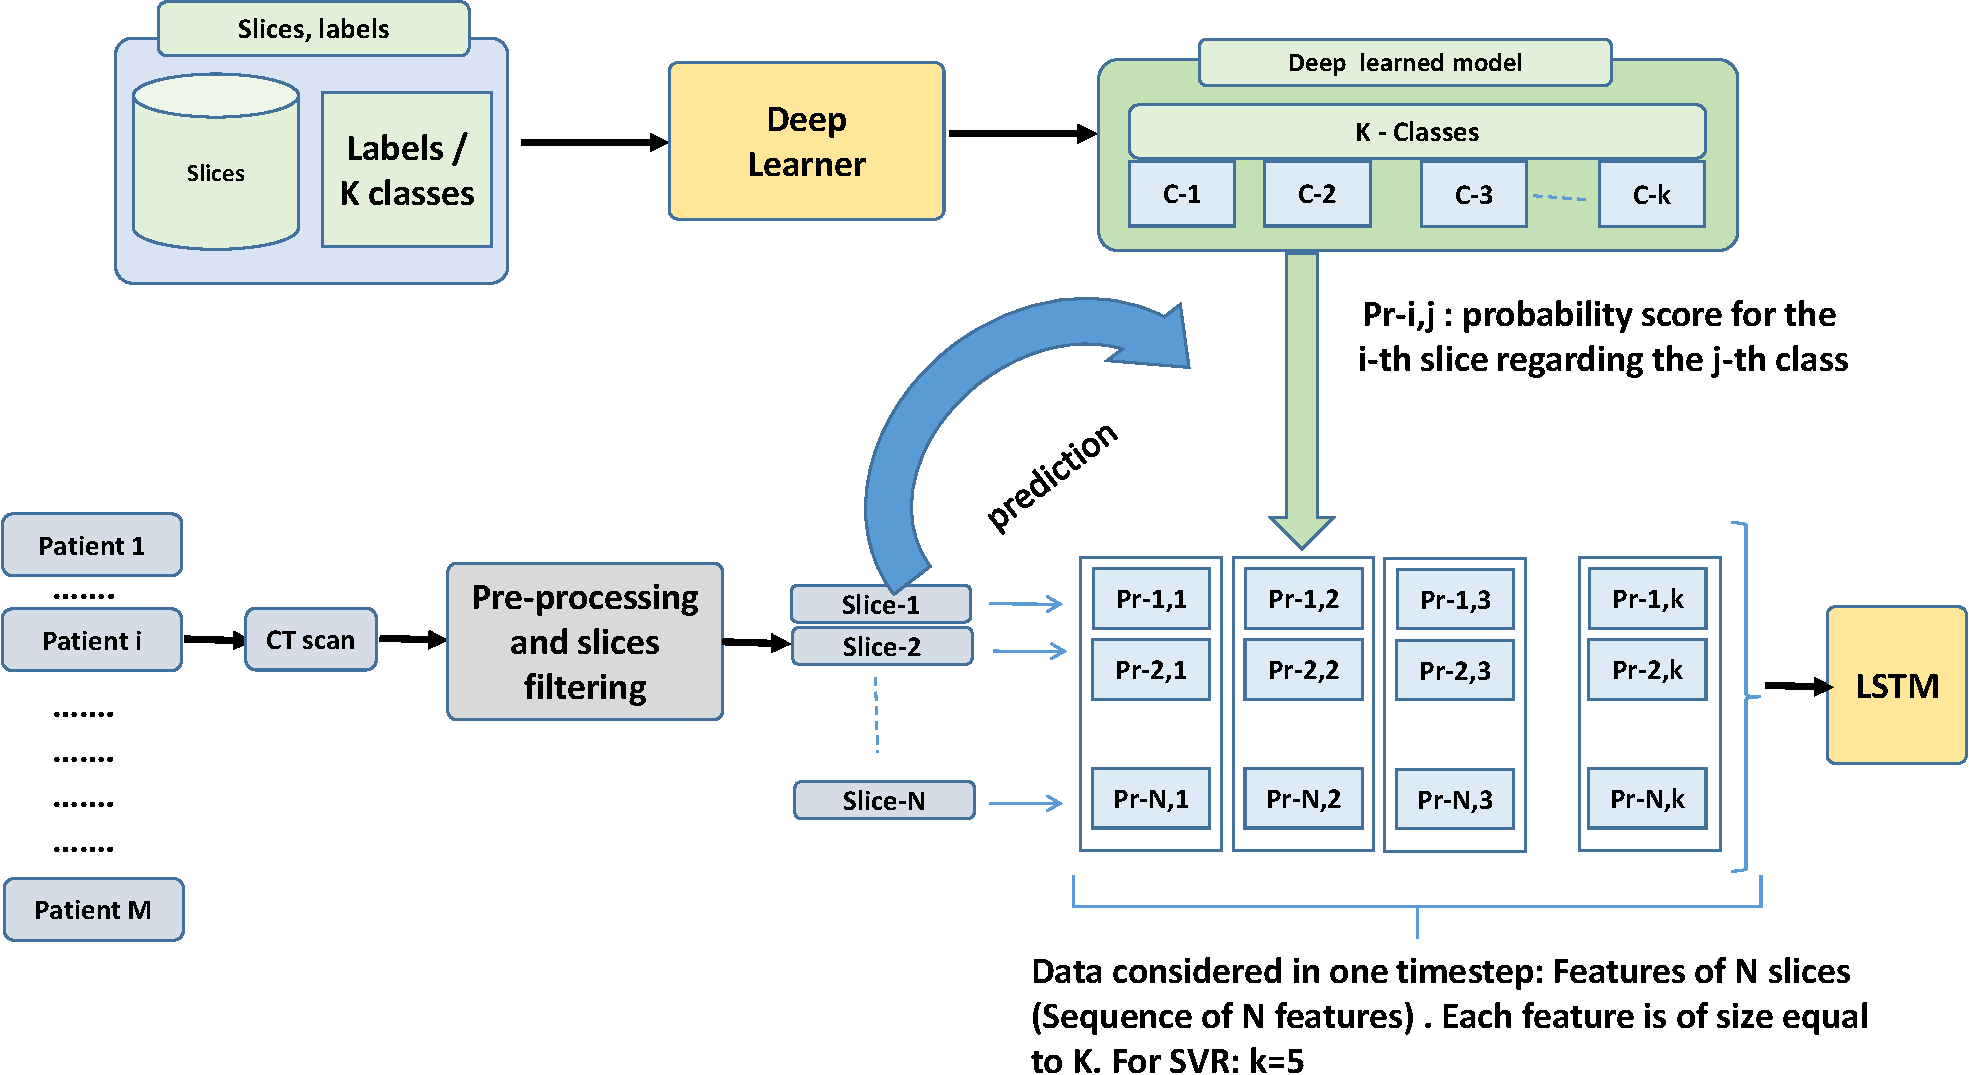
\includegraphics[width=\textwidth,height=8cm]{lstm.pdf}
\caption{Exploiting slices by LSTM as time series.} 
\label{fig:lstm}
\end{figure}

\subsection{LSTM as classification model}
\label{lstm}
As each patient is described by a sequence of slices, it is interesting to test the LSTM (Long Short-Term Memory)~\cite{lstm1997} recurrent neural network that is suitable for such data type. However, it is not recommended to apply LSTM on slices as input. Extracting features from slices using deep learner and pushing them to LSTM seems to be a good alternative. We propose to describe each slice by a feature of size equal to the number of the considered classes (five classes for SVR task). This feature is composed of the five values corresponding to the probabilities of the considered classes. These values are obtained through a deep learning stage. After generating these features, they are pushed to LSTM neural network by considering the ordered set of slices of each patient as a sequence. Figure~\ref{fig:lstm} describes the whole process.



\section{Experiments and results}
We describe in the following sections our main runs submitted to the SVR and CTR tasks.\\

We used in our experimental work the following tools:
\begin{itemize}
\item med2image~\cite{med2image} for the conversion of nifti medical images to the classic Jpeg format;
\item Tenserflow frawework~\cite{tensorflow2015} and Keras library~\cite{keras2015} for deep learning;
\item scikit-learn~\cite{scikit-learn} library for testing several machine learning techniques.

\end{itemize}

We chose to use slices of the -Z- dimension because our experiments showed that they are more suitable than those of the two other ones and got better results.

\subsubsection{Dataset:}
The dataset used in SVR task includes chest CT scans of TB patients along with some metadata regarding a set of 19 classes. 2 classes concern the SVR task, six other classes concern CTR task. The other values are considered as additional information regarding the patients that could be used as contextual information. Table~\ref{tab1} summarizes the number of CT scans for train and test collections.

\begin{table}
\center
\caption{Dataset given for Tuberculosis SVR and CTR tasks~\cite{ImageCLEF19}.}
\label{tab1}
\begin{tabular}{|l|c|c|}
\cline{2-3}
\multicolumn{1}{}{}  & 	\multicolumn{1}{|c|}{Train Collection}  &	\multicolumn{1}{|c|}{Test Collection}  \\
\hline
Number of patients 			&	218 					&		117\\
\hline
\end{tabular}
\end{table}

The same dataset is given for the CTR task. The samples are labeled regarding seven main target classes: 
\begin{enumerate}
\item Target classes for SVR Task:
\begin{enumerate}
\item SVR\_severity (binary class: HIGH and LOW). Another label called md\_Severity is given (Five discrete values ranging from 1 to 5). We remind that values of md\_Severity (1, 2 and 3) belong to the ``HIGH" Severity case. The other two values (4 and 5) correspond to the ``LOW" Severity.
\end{enumerate}
\item Target classes for CTR Task (binary classes):
\begin{enumerate}
\item Left lung affected;
\item right lung affected;
\item presence of calcifications;
\item presence of caverns;
\item presence of pleurisy;
\item lung capacity decrease.
\end{enumerate}
\end{enumerate}


\subsection{SVR task}
\subsubsection{Experimental protocol:}

We used the train collection provided by the organizers and we split it into two sub-collections: training and validation sets. We finally submitted three main runs. The other submissions concern some tested approaches that we could not optimize and finalize correctly because of luck of time:
\begin{itemize}
\item \textbf{SVR\_FSEI\_resnet50\_run3}: results of ResNet-50 trained on 50\% of training data. Each patient was represented by 50 slices filtered using the automatic unsupervised filtering approach that was described in section~\ref{preprocess}. The slices were adapted by resizing them directly using the Python Imaging Library (PIL). The input images of Resnet50 are of size $199\times199$;
\item \textbf{SVR\_FSEI\_lungnet\_run2}: results of LungNet deep learner trained on 80\% of data. Each patient was represented by 10 slices filtered using the automatic supervised filtering approach that was described in section~\ref{preprocess};
\item \textbf{SVR\_FSEI\_lstm\_run8}: results of LSTM exploiting outputs of Lungnet deep learner. Each patient was represented by 50 slices filtered using the automatic unsupervised filtering approach. So, a sequence for the LSTM learner is composed of the 50 features representing the 50 slices of the patient.
\end{itemize}

We considered for each run a hierarchical classification problem. Firstly, we classified the samples in the 5 classes corresponding to the five degrees of severity. Secondly, We deduced for each patient its predicted class using a majority vote on the predicted labels of all slices. Finally, the class predicted in the previous step is transformed to a binary value corresponding to the SVR\_Severity class (HIGH if predicted\_class $\in$ $\{1,2,3\}$ and LOW if not).\\

Our tools and scripts used in our experiments are accessible in~\cite{anouargit}.

\subsubsection{Results:}

Table~\ref{tab:resultstestsvr} shows the results in terms of AUC and accuracy obtained by our runs on the evaluation performed by the ImageCLEF committee on test collection.

\begin{table}
\center
\caption{Results on test set for SVR task.}
\label{tab:resultstestsvr}
\begin{tabular}{|l||c||c||c|}
\hline
Runs						&	AUC		& 	Accuracy	&	Rank		\\
\hline
 \textbf{SVR\_FSEI\_resnet50\_run3}			&	0.6510		&	0.6154		&	22		\\
 \textbf{SVR\_FSEI\_lungnet\_run2}			&	0.6103		&	0.5983		&	33		\\
 \textbf{SVR\_FSEI\_lstm\_run8}				&	0.6475		&	0.6068		&	25		\\
\hline
\end{tabular}
\end{table}

We can see that \textbf{SVR\_FSEI\_resnet50\_run3} got the best performance followed by  \textbf{SVR\_FSEI\_lstm\_run8}. These two runs were ranked 22th and 25th out of 54 submissions.\\

We note that for \textbf{SVR\_FSEI\_lungnet\_run2} patients were represented by 10 slices (50 slices for the two other runs), it would be interesting to see the performance of the Lungnet model within 50 slices in order to make a detailed comparison regarding the other two runs.



\begin{figure}[!ht]
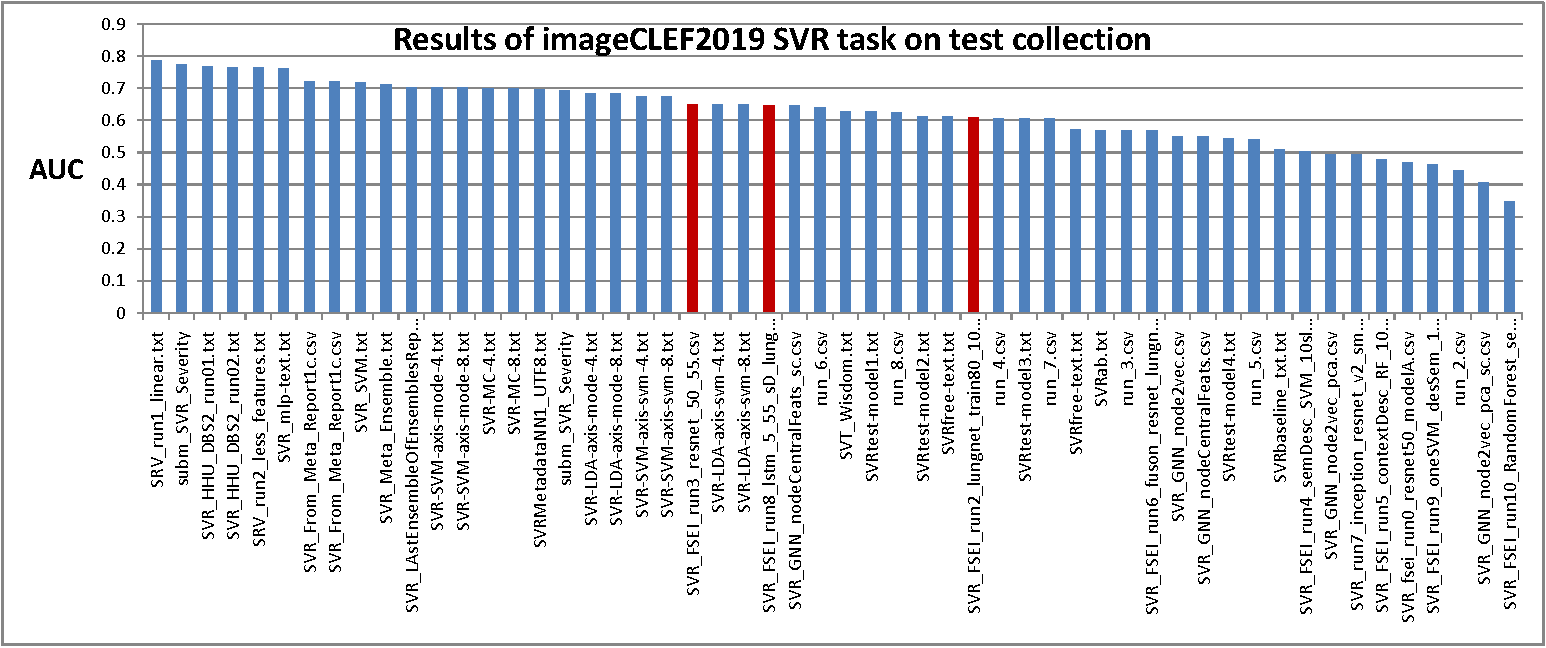
\includegraphics[width=12cm,height=8cm]{results_svr_test_auc.pdf}
\caption{Results and ranking in terms of AUC on test data for SVR Task.} 
\label{fig:svrresultstestauc}
\end{figure}

Figures~\ref{fig:svrresultstestauc} and~\ref{fig:svrresultstestaccuracy} describe the results and ranking of all submissions of SVR task in terms of AUC and accuracy, respectively. 


\begin{figure}[!ht]
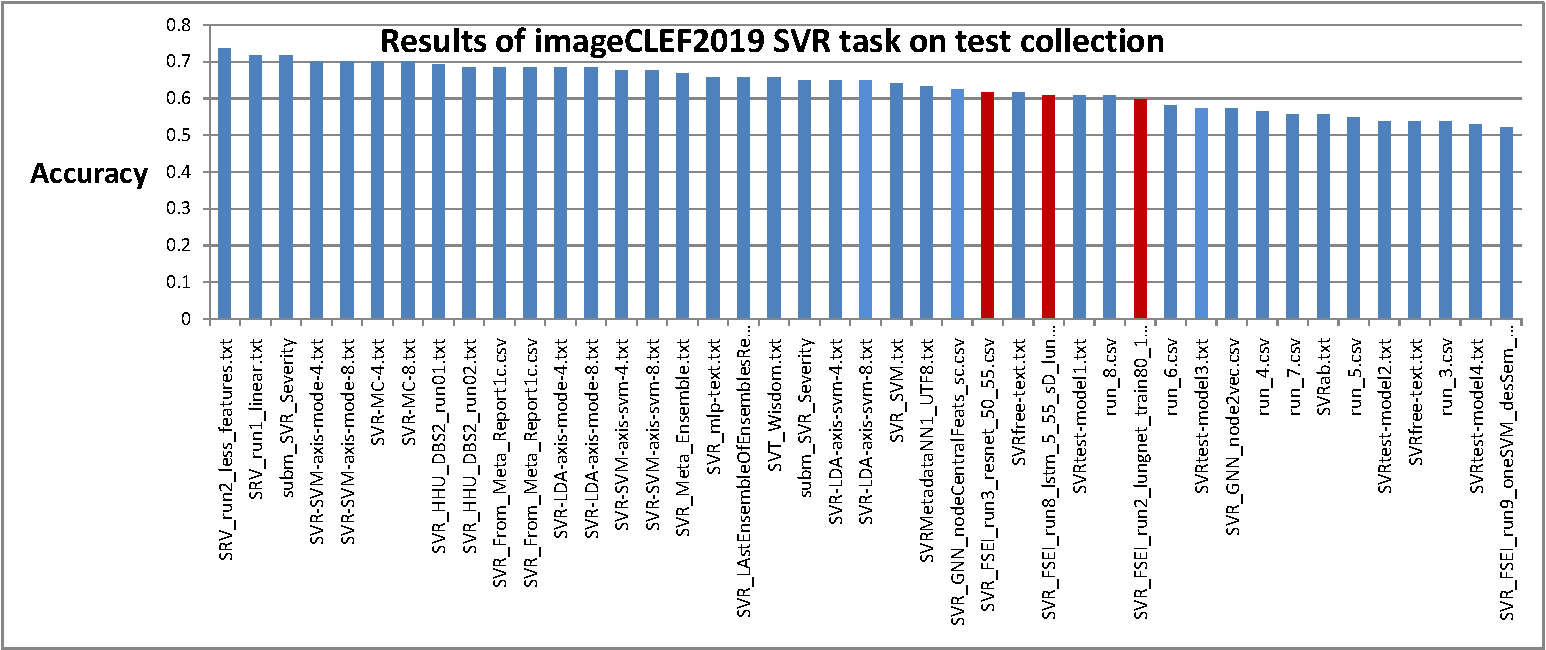
\includegraphics[width=12cm,height=7cm]{results_svr_test_accuracy.pdf}
\caption{Results and ranking in terms of Accuracy on test data for SVR Task} 
\label{fig:svrresultstestaccuracy}
\end{figure}

Although the results achieved by our submissions are not well ranked compared to those of the top of the list, we can notice that several runs belong to the same teams that had good results, and they probably do not differ too much. On the other hand, We believe that our models could give better results after a more advanced data preprocessing including the use of masks, samples selection and data augmentation.





\subsection{CTR task}
\subsubsection{Experimental protocol:}

We trained in a first step our deep models (Resnet and Lungnet). Secondly, we generated the semantic descriptors following the approach described in section~\ref{contribution}. We treated the problematic as a multi-class problem in the first learning stage and as a binary classification problem in the second learning step. We used in the latter SVM as a binary classifier. We optimized its parameters independently for each target class.\\

We submitted three main runs:
\begin{enumerate}
\item  \textbf{CTR\_FSEI\_run1}:  results of LungNet trained on 50\% of training data. Each patient was represented by 10 slices filtered using the automatic supervised filtering approach that was described in section~\ref{preprocess};
\item  \textbf{CTR\_FSEI\_run2} :  results of LungNet trained on 70\% of training data. Each patient was represented by 50 slices filtered using the automatic unsupervised filtering approach that was described in section~\ref{preprocess};
\item  \textbf{CTR\_FSEI\_run5}: SVM using semantic features. The latter are extracted using Resnet-50 as deep learner. Each patient was represented by 10 slices filtered using the automatic supervised filtering approach that was described in section~\ref{preprocess}.\\
\end{enumerate}

Our tools and scripts used in our experiments are accessible in~\cite{anouargit}.

\subsubsection{Results:}


Table~\ref{tab:resultstestctr} shows the results (in terms of Average-AUC and Min-AUC) and ranking obtained by our runs on the evaluation performed by the ImageCLEF committee on test collection.\\

\begin{table}
\center
\caption{Results on test set for CTR task.}
\label{tab:resultstestctr}
\begin{tabular}{|l||c||c||c|}
\hline
Runs					&	Mean AUC	&	Min AUC	&	Rank		\\
\hline
CTR\_FSEI\_run1				& 	0.6273		&	0.4877	&	14		\\
CTR\_FSEI\_run2				& 	0.6061		&	0.4471	&	17		\\
CTR\_FSEI\_run5				& 	0.5064		&	0.4134	&	32		\\
\hline
\end{tabular}
\end{table}

We can see that our best results were obtained by  \textbf{CTR\_FSEI\_run1} followed by  \textbf{CTR\_FSEI\_run2}. However, we should mention here that we used the same sub-division of the corpus in two sub-parts (train and validation) for all CTR target classes, which is not optimal since the distribution of class values is not the same for the six target classes. This explains the disadvantage of the run \textbf{CTR\_FSEI\_run5} compared to the other two and also the low value of Min-AUC for the three runs. We believe that the semantic descriptors approach might perform better by making more efforts to optimize parameters or by testing another learner like the Bagging of Random Forests as presented in~\cite{HamadiY18}. Considering a multi-label classifier constitutes also an interesting idea to test.\\

Figure~\ref{fig:ctrresultsauc} describes the results (in terms of Average-AUC) and ranking of all submissions of CTR task. Our best two runs were ranked 14th and 17th out of 35 submissions.\\

\begin{figure}[!ht]
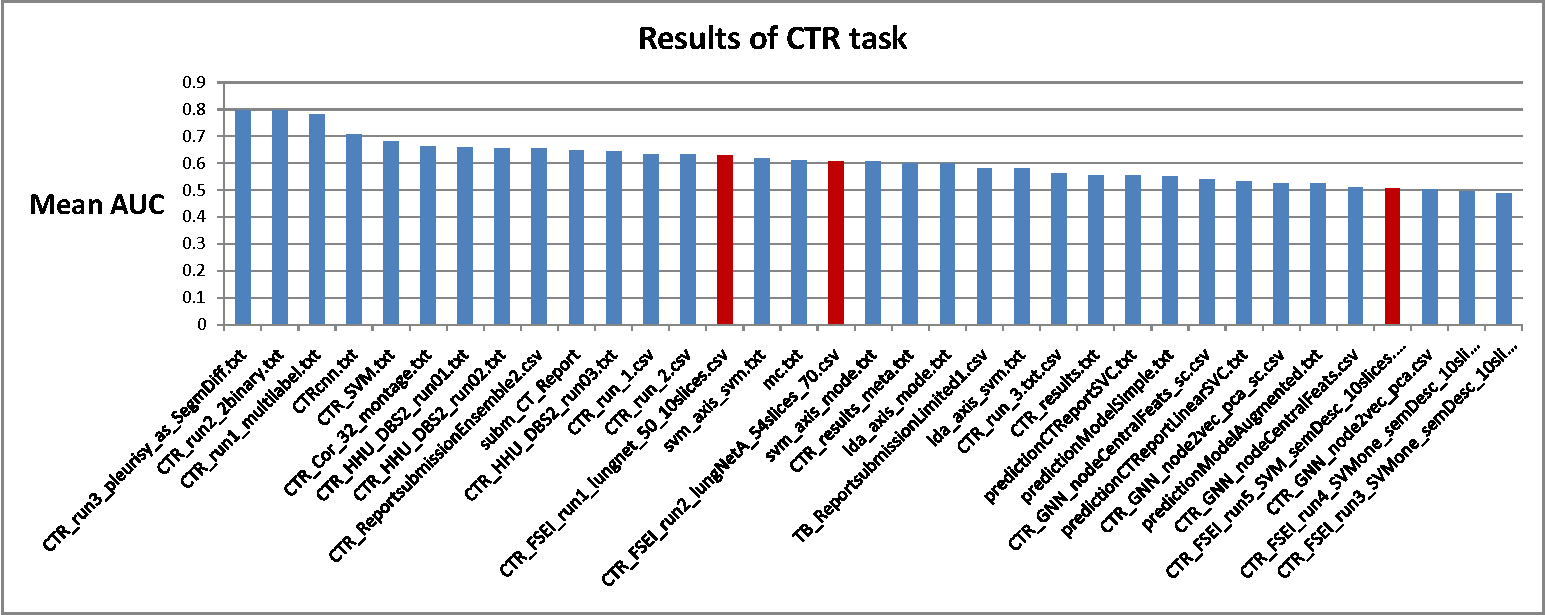
\includegraphics[width=12cm,height=8cm]{results_ctr_test_meanauc.pdf}
\caption{Results and ranking in terms of Mean-AUC on test collection for CTR Task.} 
\label{fig:ctrresultsauc}
\end{figure}


\section{Conclusion and future works}

We have described in this article our contributions to the SVR and CTR sub-tasks of ImageCLEFmed 2019 Tuberculosis task. We proposed to use after a data preprocessing step, a deep learner to classify samples in the target classes. We used for that ResNet-50 and proposed our LungNet architecture. Moreover, we proposed to extract a single semantic descriptor for each CT image / patient instead of considering all the slices as separate samples. We tested also LSTM as another alternative. Although our proposals had not been the best, the results obtained showed that these approaches could be much more efficient and might give more interesting results if they are applied in an optimized way.\\

As perspectives, we plan to adopt enrichment strategies and learning samples selection. In addition, we noticed during the sub-sampling of our data that the deletion or addition of some samples had an impact on the results. On the other hand, filtering slices in an optimized way is a key idea that could further improve system performance. Furthermore, we noticed in our experiments that there is a difference in terms of precision achieved for each studied class. Indeed, some classes are more difficult to identify than others. This is also an interesting track to study. The use of masks and tracking the visual contents of lungs could also be a good trail to explore.

 \bibliographystyle{splncs04}     % mathematics and physical sciences
\bibliography{ref}


\end{document}
